
\section{Combinando clases de atributos}

Combinando los tipos de atributos definidos pudimos apreciar cuánto aporta cada clase de los mismos. Realizamos todas las combinaciones de cada uno de los tipos de atributos. Estos son: silábicos, fonéticos y acústicos. Para cada una de esas combinaciones, corrimos los clasificadores NaiveBayes y Function SMO, que son los que mejores resultados arrojaron. Las instancias utilizadas para estos tests fueron las del cross-validation generado anteriormente. En la tabla \ref{comb_atrib} y en la figura \ref{comb_atrib_graf} se puede apreciar los resultados. Cabe aclarar que los valores de la tabla surgieron del promedio de los resultados de los 5 tests generados.  

%poner tabla: FON, SIL, ACU y sus combinaciones para clasificacion 

%Datos: {'bayes.NaiveBayes': {'SIL + FON + ACU': 70.0, 'SIL + ACU': 67.0, 'FON + ACU': 71.0, 'ACU': 68.0, 'FON': 69.0, 'SIL + FON': 69.0, 'SIL': 66.0}, 'functions.SMO': {'SIL + FON + ACU': 73.0, 'SIL + ACU': 70.0, 'FON + ACU': 71.0, 'ACU': 69.0, 'FON': 65.0, 'SIL + FON': 66.0, 'SIL': 66.0}}

\begin{table}[H]
\centering
\begin{tabular}{|l|c|c|}
\hline
\textbf{} & \textbf{NaiveBayes} & \textbf{Functions SMO}   \\ \hline
SIL + FON + ACU & 70 \% & 73 \% \\ \hline
SIL + FON & 69 \% & 66 \% \\ \hline
FON + ACU & 71 \% & 71 \% \\ \hline
SIL + ACU & 67 \% & 70 \% \\ \hline
ACU & 68 \% & 69 \% \\ \hline
SIL & 66 \% & 66 \% \\ \hline
FON & 69 \% & 65 \% \\ \hline
\end{tabular}
\caption{Combinación de atributos y su resultado}
\label{comb_atrib}
\end{table}

\begin{figure}[H]
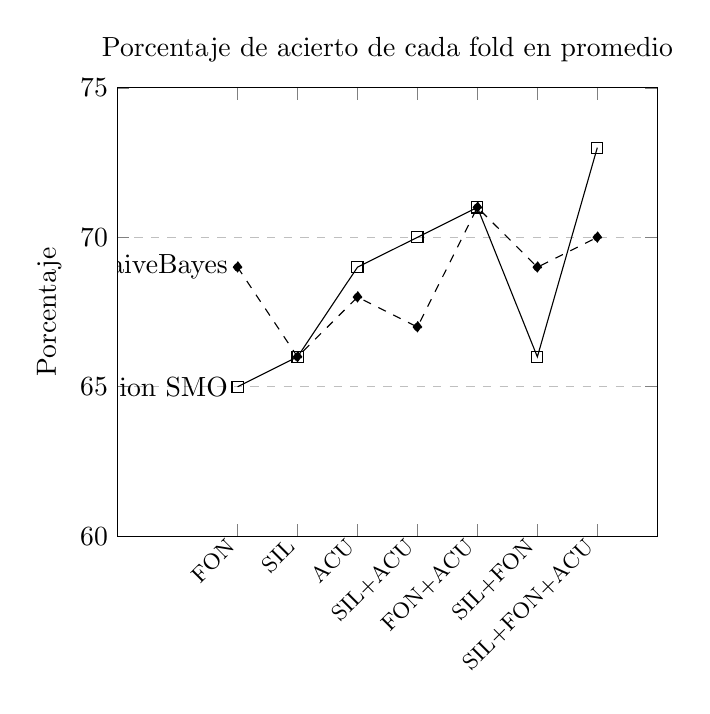
\begin{tikzpicture}

\begin{axis}[
    title={Porcentaje de acierto de cada fold en promedio},
    ylabel={Porcentaje},
    xmin=-1, xmax=8,
    ymin=60, ymax=75,
    xtick={1,2,3,4,5,6,7},
    xticklabels={FON,SIL,ACU,SIL+ACU,FON+ACU,SIL+FON, SIL+FON+ACU},
    x tick label style={rotate=45, anchor=east, font=\footnotesize},
    ytick={60,65,70,75},
    ymajorgrids=true,
    grid style=dashed,
] 

\addplot[mark=diamond*,dashed]coordinates {
    (1,69)(2,66)(3,68)(4,67)(5,71)(6,69)(7,70) };
\addplot[mark=square,solid,]coordinates {
    (1,65)(2,66)(3,69)(4,70)(5,71)(6,66)(7,73) };

\node [left] at (axis cs: 1, 69) {NaiveBayes};
\node [left] at (axis cs: 1, 65) {Function SMO};

\end{axis}
\end{tikzpicture}
\caption{Gráfico combinando distintos grupos de atributos}
\label{comb_atrib_graf}
\end{figure}

Lo esperable es que aumentando la cantidad de atributos se aumente el porcentaje de instancias  clasificadas correctamente. Esta idea se comprueba ya que la combinación que obtuvo mejor porcentaje fue $SIL+FON+ACU$ para el clasificador Function SMO. En segundo lugar salió la combinación de $FON+ACU$ para ambos clasificadores y en tercero $SIL+ACU$ sólo para Function SMO. 

Podemos notar que el tipo de atributo que posee mayor presencia es el que corresponde a los atributos acústicos ($ACU$), ya que se encuentran en los tres primeros grupos de atributos que obtuvieron mejor porcentaje (estos son: $SIL+FON+ACU$, $FON+ACU$ y $SIL+ACU$). Quizás entre los atributos acústicos no haya uno con información predominante, pero la combinación de todos los atributos de esa clase hace que los clasificadores tengan buenas métricas.